\graphicspath{{./chapter/beamer/figures/}}
% ------------------------------------------------------------------------
\chapter{Beamer Helper}

Beamer allows the creation of presentations based on the \LaTeX document creation platform. This document contains a short introduction on how to use Beamer, including a tutorial on how to install and use \textit{pympress}.

\section{Intro to Beamer presentations}

Beamer presentations use the beamer document class, ie. the document must start with
\textcolor{blue}{$\backslash$documentclass}\textcolor{orange}{\{beamer\}},
other than a few other beamer specific options, the preamble is equivalent to any other \LaTeX document.
\par
Slides are declared by the frame environment, all content that is meant to be shown should be declared inside this environment. Slides will appear in the order they are declared.

\section{Adding presenter notes to beamer}

Presenter notes are added by the
\textcolor{blue}{$\backslash$note}\textcolor{orange}{\{slide notes\}}
command. This command is declared outside the frame environment and by default adds notes to the previous frame environment (if necessary this can be altered with the appropriate options). Combined with the itemize option, the note command can be called as
\\
\textcolor{blue}{$\backslash$note[itemize]}\textcolor{orange}{\{\\
\textcolor{blue}{$\backslash$item} item 1\\
\textcolor{blue}{$\backslash$item} item 2\\
...\\
\}}
\par
The notes are not displayed by default, the option \textcolor{blue}{$\backslash$setbeameroption}\textcolor{orange}{\{show notes on second screen\}}
should be added in the preamble of the document. The notes will then appear appended to the right of every slide, an example of this can be seen in Figure~\ref{fig:slidesAndNotesExample}. These note slides are flagged, so using an appropriate program (for example \textit{pympress}) it is possible to achieve a presenter view, displaying the notes and slide proper on different windows/screens.

\begin{figure}[h]
\centering
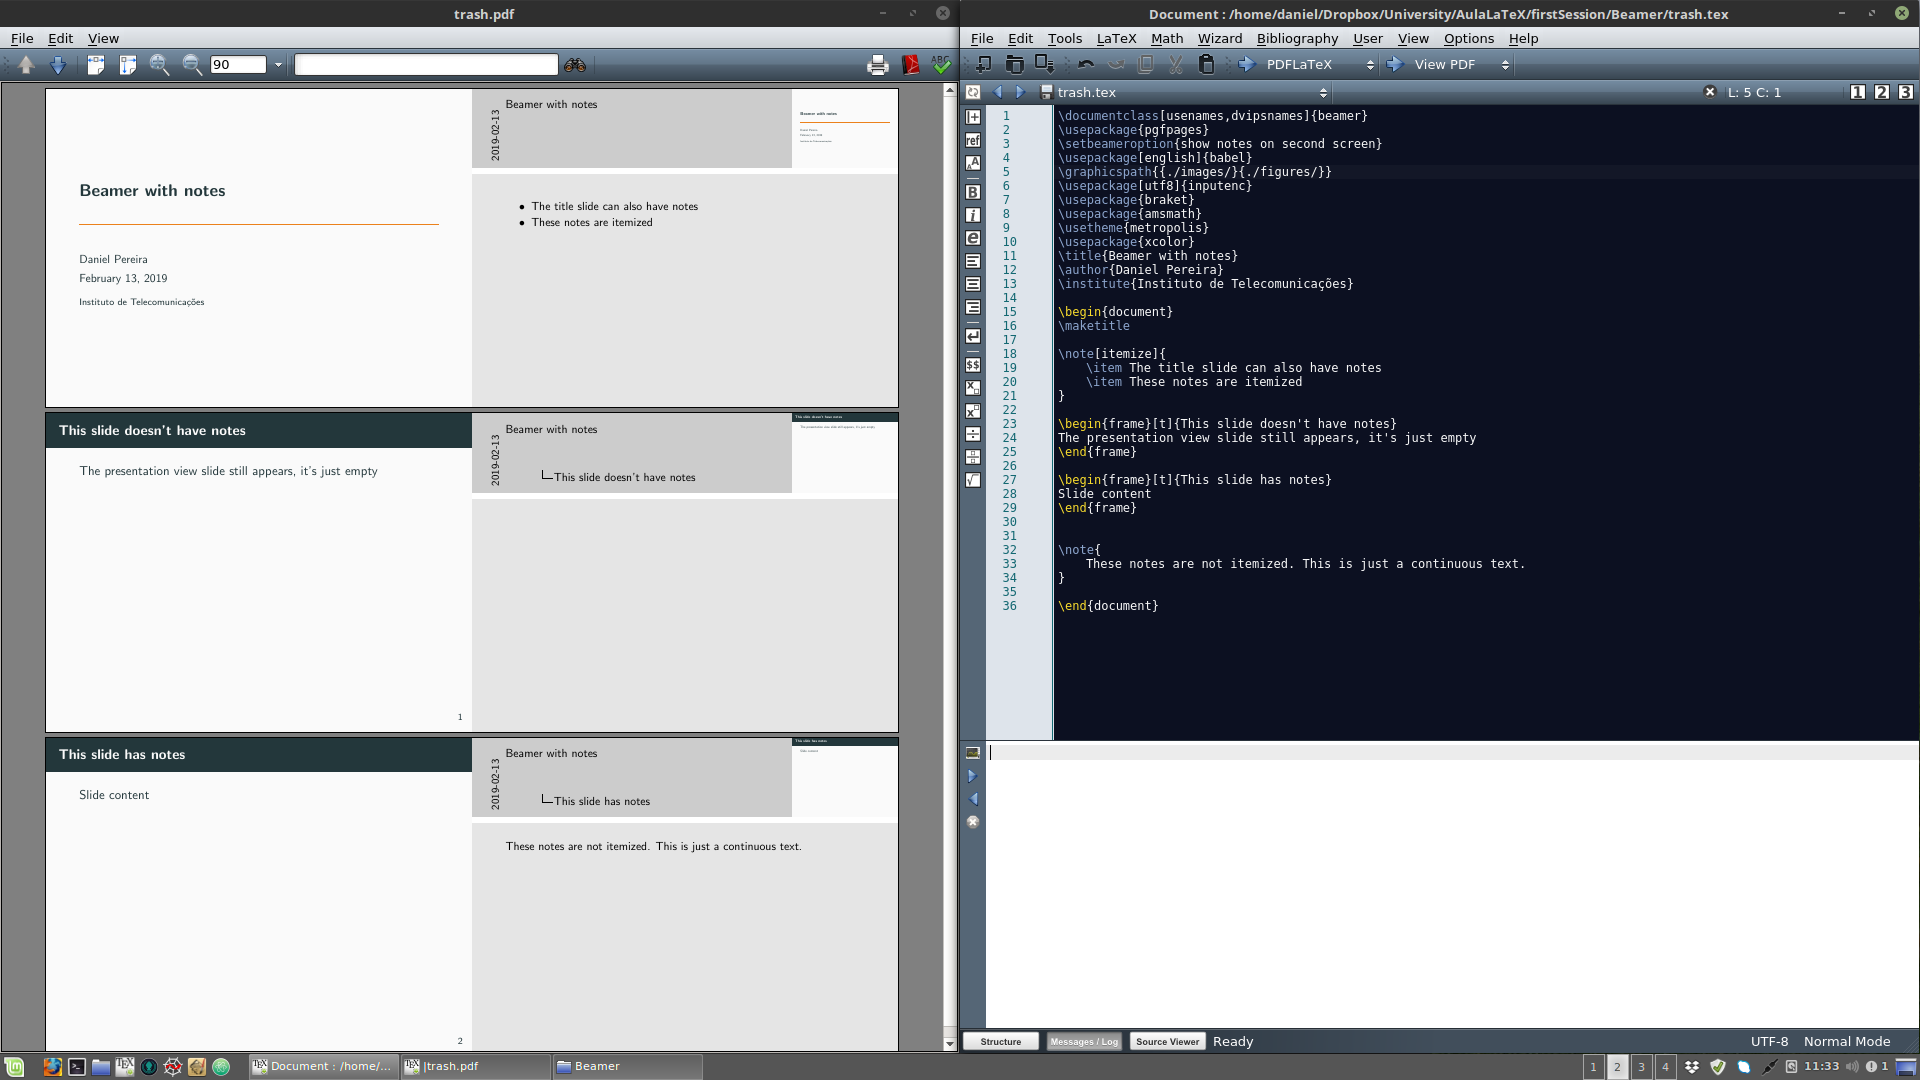
\includegraphics[width=\linewidth]{codeANDslideEXAMPLE.png}
\caption{Example of a Beamer presentation with presentation notes.}
\label{fig:slidesAndNotesExample}
\end{figure}

\subsection{Installing and using \textit{pympress}}

Pympress is a multiplatform, python based PDF reader designed specifically for dual-screen presentations, available at \url{https://github.com/Cimbali/pympress}. Installers for Windows are available at \url{https://github.com/Cimbali/pympress/releases/tag/v1.2.0}, these also deal with all the dependencies and are thus the recommended method for Windows machines.
\par
For non-Windows machines the install process can be more involved and the precise steps may vary from machine to machine. First of all, the following dependencies are required
\begin{itemize}
\item Python 2.7 or 3.x, installed from \url{https://www.python.org} preferably, so as to include the \textit{pip} package manager.
\item Poppler
\item Gtk+ 3 and the following sub-dependencies
\begin{itemize}
\item Cairo
\item Gdk
\end{itemize}
\item PyGi
\item optional: VLC
\end{itemize}
more information on the installation of the dependencies can be found in \url{https://github.com/Cimbali/pympress#dependencies}.
\par
After all the the dependencies have been installed, \textit{pympress} is installed through the command
\begin{verbatim}
pip install pympress
\end{verbatim}
\par
On Windows, \textit{pympress.exe} can be used to run the program, from which you can then open the presentation PDF as with a regular PDF reader, this executable should be in /ProgramFiles/pympress/. On Linux \textit{pympress} is run from the terminal, either by calling
\begin{verbatim}
pympress
\end{verbatim}
in which case \textit{pympress} is opened without a PDF file, the presentation can then be openned from inside \textit{pympress}.
In both of the previous situations, \textit{pympress} opens as in Figure~\ref{fig:pympressColdOpen}
\begin{figure}[h]
\centering
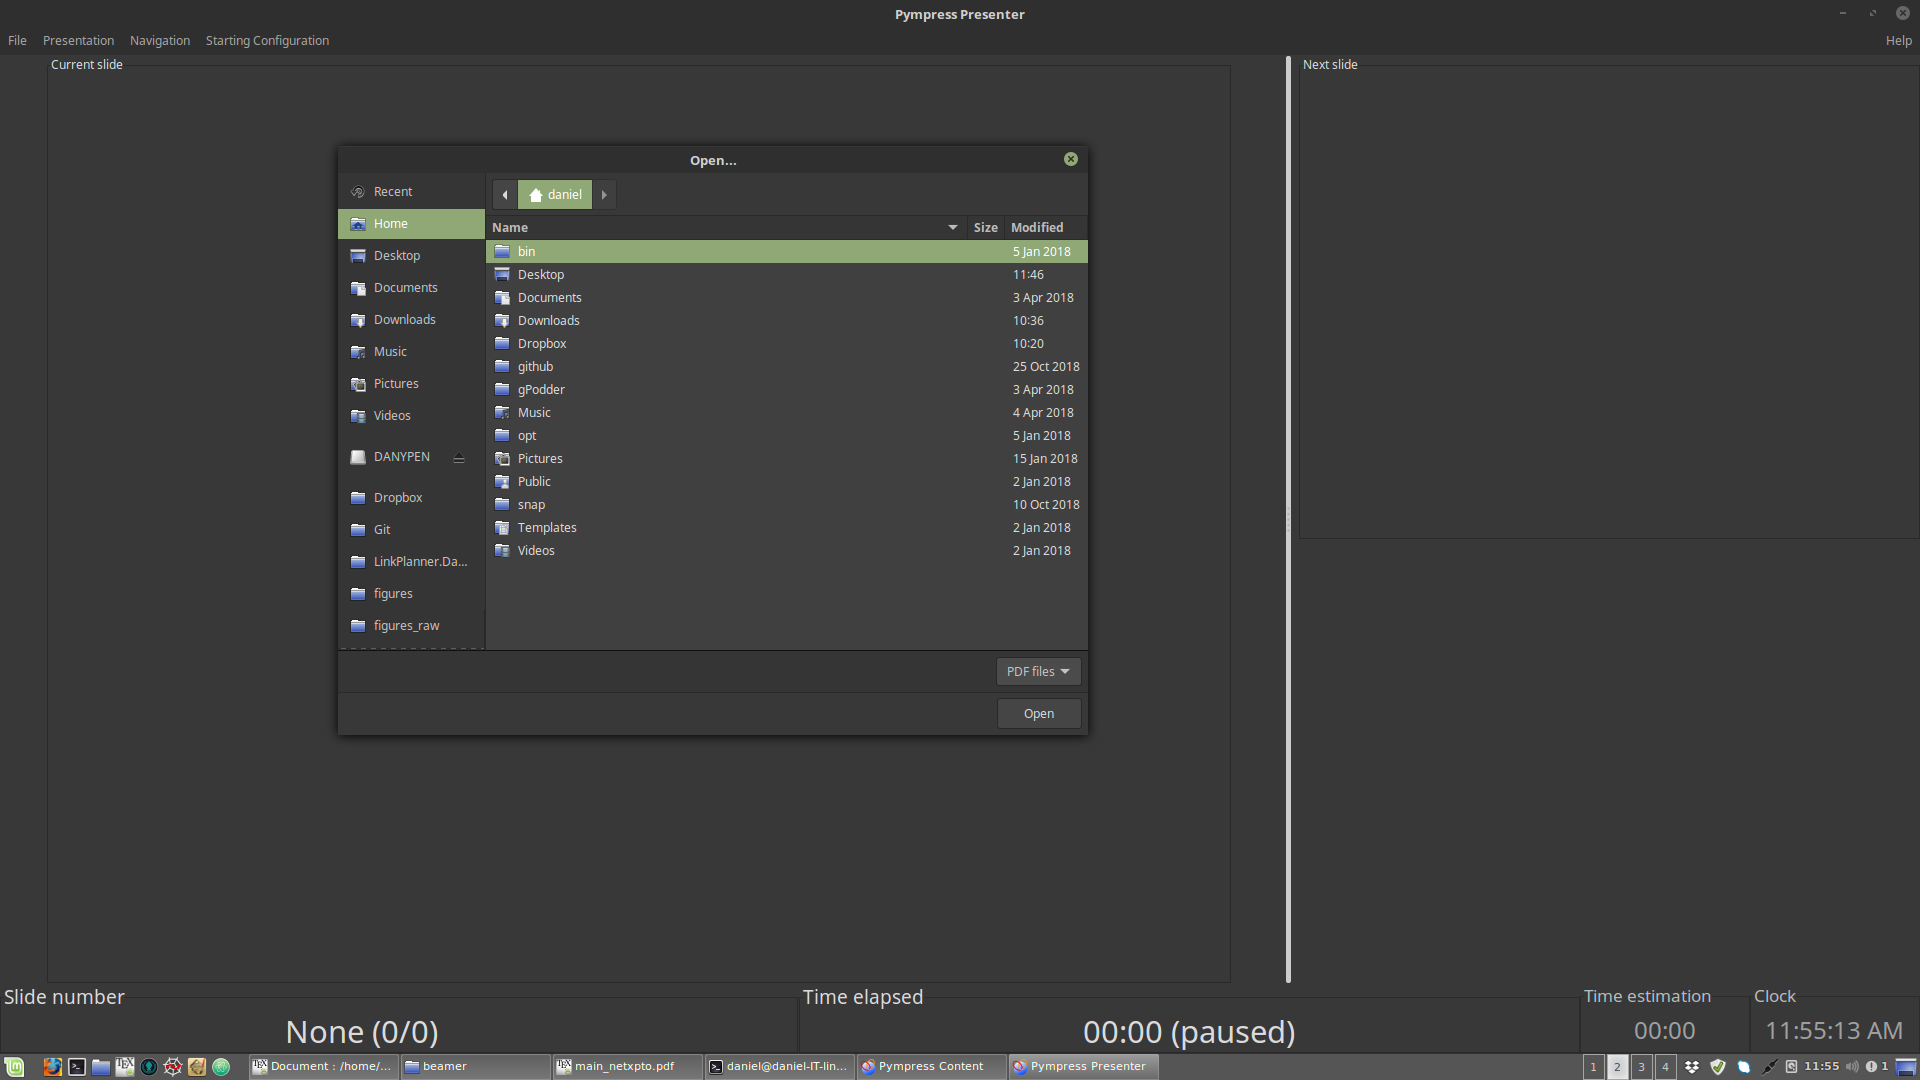
\includegraphics[width=.7\linewidth]{pympressColdOpen.png}
\caption{Example of \textit{pympress} open without a PDF presentation.}
\label{fig:pympressColdOpen}
\end{figure}
\par
Alternatively, the presentation can be opened directly from the terminal by navigating to the folder with the PDF file and calling
\begin{verbatim}
pympress presentationFileName.pdf
\end{verbatim}
The presenter view includes multiple functionalities, available from the menus in the menu bar. An example of \textit{pympress} opened with a presentation can be seen in Figure~\ref{fig:pympressPresentation}.
\begin{figure}[h]
\centering
\begin{subfigure}{.49\linewidth}
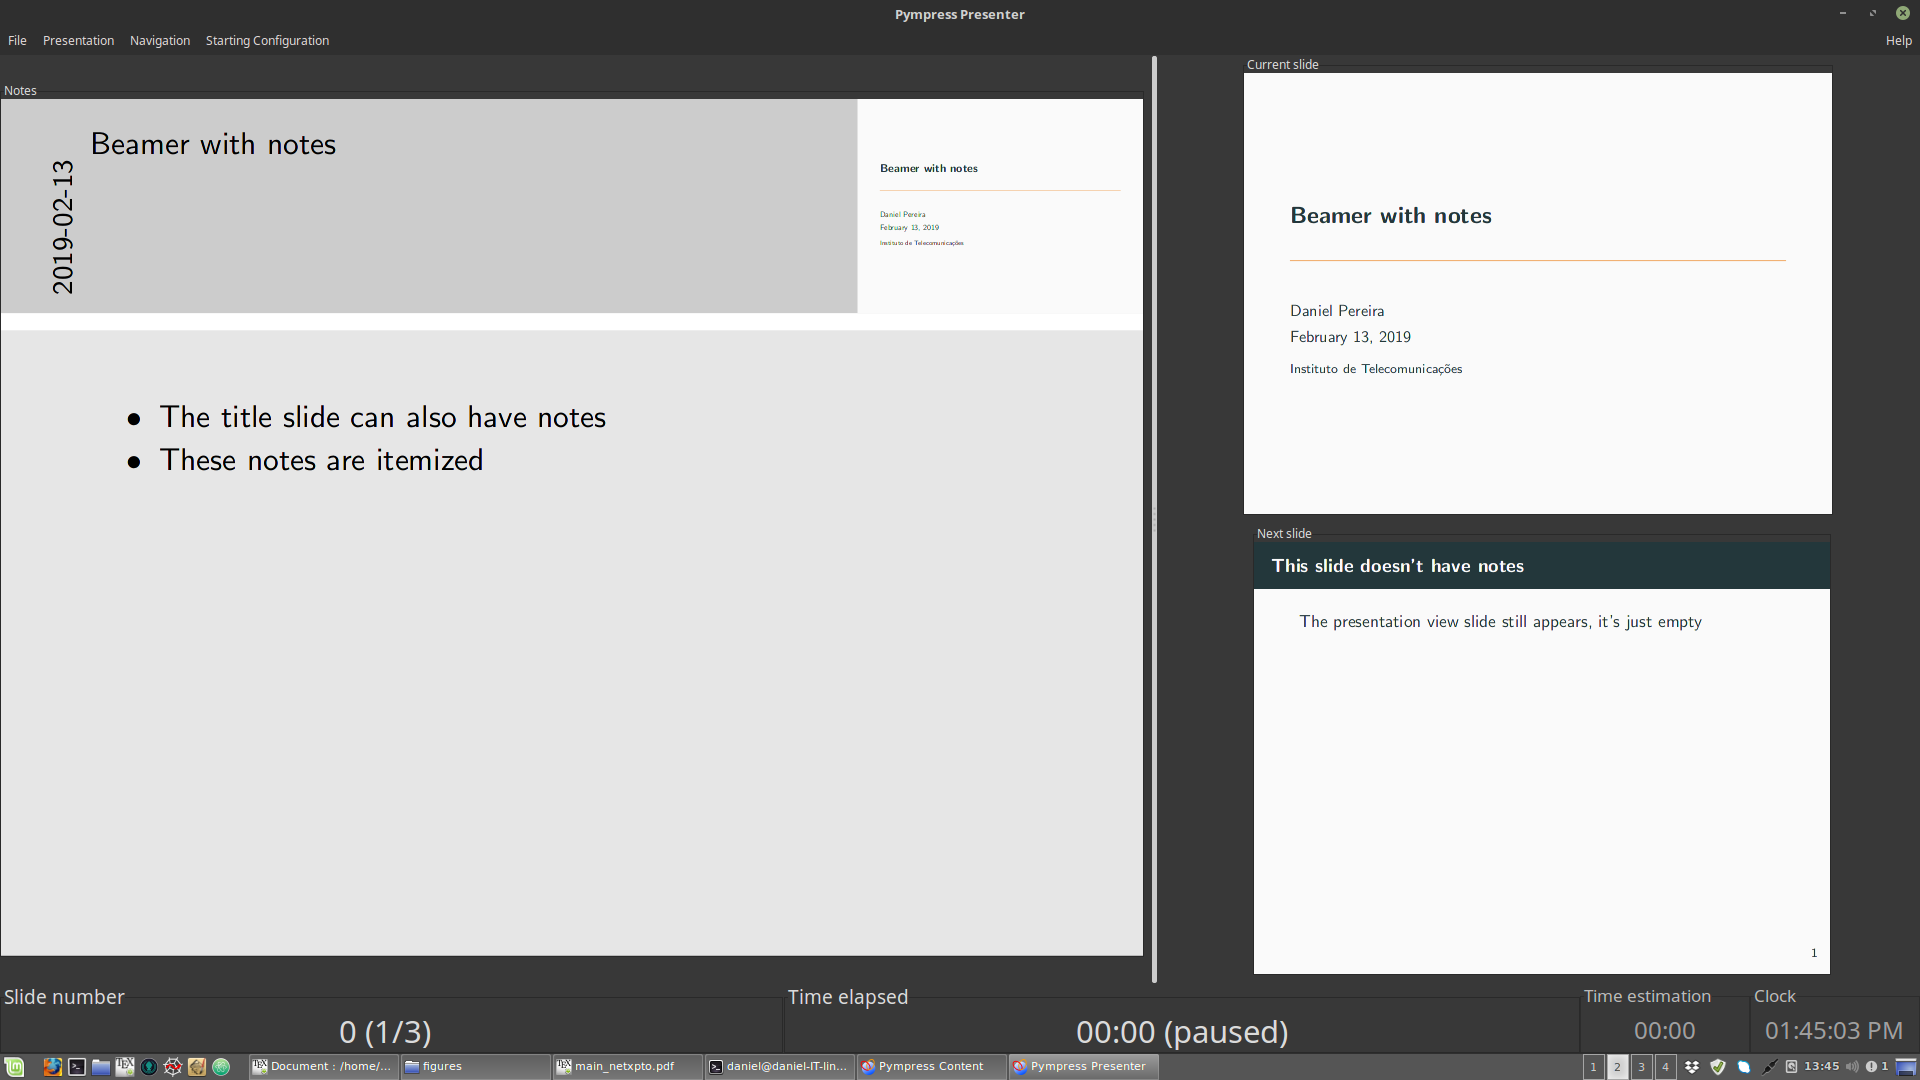
\includegraphics[width=\linewidth]{presentatorView.png}
\end{subfigure} ~
\begin{subfigure}{.49\linewidth}

\includegraphics[width=\linewidth]{presentation.png}
\end{subfigure}
\caption{Example of \textit{pympress} presenter view (left) and corresponding presentation (right).}
\label{fig:pympressPresentation}
\end{figure}
	

\section{IT template}
